% 页面配置文件（中南大学实验报告模板 A4竖版有框）

% A4竖版高度为29.7cm，宽度为21.0cm

\documentclass[xiaosi]{ctexart}

% --- 页面与布局设置 ---
\usepackage[a4paper]{geometry}
\geometry{
	top=1.6cm, % 调整上边距
	bottom=1.6cm, % 调整下边距
	left=2.5cm, % 调整左边距
	right=2.0cm % 调整右边距
}
\setlength{\parindent}{2em}

% --- 字体设置 ---
\usepackage{xeCJK}
\usepackage{fontspec}
\usepackage{unicode-math}
% 设置中文字体
\setCJKmainfont{SimSun}      % 正文宋体
\setCJKsansfont{SimHei}      % 无衬线黑体
\setCJKmonofont{FangSong}    % 等宽仿宋 (可自行修改)
\setmainfont{Times New Roman} % 设置英文字体
\setmathfont{XITS Math} % 设置数学公式字体

% --- 宏包引入 ---
\usepackage{graphicx}       % 用于插入图片
\usepackage{titlesec}       % 用于自定义标题格式
\usepackage{zhnumber}       % 用于将数字转为中文序号
\usepackage{amsmath}        % AMS数学公式宏包
\usepackage{framed}         % 用于给正文加边框
\usepackage{tikz}           % 用于绘制装订线
\usepackage{eso-pic}        % 用于在页面固定位置放置内容
\usepackage{indentfirst}
\usepackage{caption}
\usepackage{setspace}
\usepackage{booktabs}
\usepackage{float}
\usepackage{listings} % listings 宏包用于代码高亮
\usepackage{xcolor} % xcolor 宏包用于设置代码颜色

% --- 页面样式与路径设置 ---
\pagestyle{empty} % 全文不显示页码
\graphicspath{{./picture/}} % 设置图片都存放在./picture/文件夹内

% --- 装订线设置 ---
% 使用eso-pic和tikz在每一页的左侧绘制虚线和文字“装订线”
\AddToShipoutPictureBG{
	\AtPageLowerLeft{
		\begin{tikzpicture}[remember picture, overlay]
			% 装订线位于左页边距3cm的中间位置
			\coordinate (start) at (1.25cm, 1.5cm); 
			\coordinate (end) at (1.25cm, 28.2cm);
			\draw[dashed] (start) -- (end);
			\node[rotate=90, anchor=south, font=\small] at (1.25cm, 14.85cm)
			{装\hspace{6em}订\hspace{6em}线};
		\end{tikzpicture}
	}
}

% --- 设置 listings 代码（代码块）样式 ---
\lstset{
	language=Python, % 设置默认语言为 Python
	basicstyle=\ttfamily\zihao{-5}, % 字体为等宽字体 (Typewriter)，五号字
	lineskip={0.5ex}, % 微调行间距，可根据效果调整
	keywordstyle=\color{blue}\bfseries, % 关键字颜色为蓝色，加粗
	commentstyle=\color[rgb]{0.0, 0.5, 0.0}\itshape, % 注释颜色为深绿，斜体
	stringstyle=\color[rgb]{0.7, 0.0, 0.0}, % 字符串颜色为深红
	showstringspaces=false, % 不显示字符串中的空格
	frame=single, % 添加单线边框
	framesep=5pt, % 边框与代码的间距
	rulesepcolor=\color{gray}, % 边框线的颜色
	backgroundcolor=\color[rgb]{0.95,0.95,0.95}, % 背景颜色为浅灰色
	breaklines=true, % 自动断行
	tabsize=4, % 制表符宽度
	numbers=left, % 显示行号
	xleftmargin=2em, % 代码框左侧留出2em空间
	xrightmargin=2em % 代码框右侧留出2em空间
}

% --- 调整公式行间距---
% 减小公式上方间距（长行）
\setlength{\abovedisplayskip}{1pt plus 0.5pt minus 0.5pt}
% 减小公式下方间距（长行）
\setlength{\belowdisplayskip}{1pt plus 0.5pt minus 0.5pt}
% 减小公式上方间距（短行）
\setlength{\abovedisplayshortskip}{1pt plus 0.5pt minus 0.5pt}
% 减小公式下方间距（短行）
\setlength{\belowdisplayshortskip}{1pt plus 0.5pt minus 0.5pt}

% --- 标题格式定义 ---
% 一级标题 (例如: 一、实验目的)
% 格式: 三号、黑体, 靠左, 缩进1个字符
\renewcommand{\thesection}{\zhnum{section}}
\titleformat{\section}
{\normalfont\heiti\zihao{3}} % 字体格式
{\thesection、}              % 标题编号
{0em}                      % 编号与标题文字的间距
{}                         % 标题前的代码
\titlespacing*{\section}
{1em}   % 左边距 (缩进1字符)
{3ex}    % 标题前间距
{2ex}    % 标题后间距

% 二级标题
% 格式: 小四、黑体, 靠左, 缩进2个字符, 需要编号
\renewcommand{\thesubsection}{（\zhnum{subsection}）}
\titleformat{\subsection}
{\normalfont\heiti\zihao{-4}}
{\thesubsection}
{0em}
{}
\titlespacing*{\subsection}{2em} {0.5ex} {0.5ex}

% 三级标题
% 格式: 小四、楷体, 靠左, 缩进2个字符, 需要编号
\titleformat{\subsubsection}
{\normalfont\kaishu\zihao{-4}}
{\thesubsubsection}
{1em}
{}
\titlespacing*{\subsubsection}{2em} {0ex} {0ex}

% --- 图表标题设置 ---
\captionsetup[figure]
{
	font={small},
	labelsep=space,
	name={图},
	position=below,
	skip=5pt
}
\captionsetup[table]
{
	font={small},
	labelsep=space,
	name={表},
	position=above,
	skip=3pt
}

% --- 多级列表设置 ---
\usepackage{enumitem} % 引入列表控制宏包
\setlist[enumerate, 1]{ % 有序列表
	topsep=0pt,
	partopsep=0pt, % 设置列表和周围文字的间距为0
	itemsep=0pt, % 设置列表项之间的间距为0
	parsep=0pt, % 设置列表项内段落之间的间距
	labelsep=0.5em,	% 调整列表项的标签与文本的间距使其看起来更自然
	leftmargin=3.5em % enumerate列表缩进3.5em
}
\setlist[itemize, 1]{ % 无序列表
	label={·},
	topsep=0pt,
	partopsep=0pt, % 设置列表和周围文字的间距为0
	itemsep=0pt, % 设置列表项之间的间距为0
	parsep=0pt, % 设置列表项内段落之间的间距
	labelsep=0em, % 调整列表项的标签与文本的间距使其看起来更自然
	leftmargin=3.5em % itemize列表缩进3.5em
}

\begin{document}
	
	{
		\renewcommand\arraystretch{2}
		\noindent 
		\begin{tabular}{|c|c|}
			\hline
			\fangsong\hspace{0.5em}评阅人\hspace{0.5em} & \hspace{6em} \\ 
			\hline
		\end{tabular}
		\hfill 
		\begin{tabular}{|c|c|}
			\hline
			\fangsong 实验成绩 & \hspace{6em} \\ 
			\hline
		\end{tabular}
	}
	\renewcommand\arraystretch{1} 
	\vspace{2em}
	
	\begin{center}
		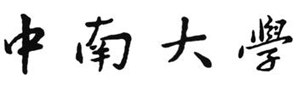
\includegraphics[width=0.5\linewidth]{csu_logo.png} 
	\end{center}
	
	\vspace{0.5em}
	
	\begin{center}
		\parbox{12.86cm}{
			\centering\heiti\zihao{0}\scalebox{0.6}[1]{
				自
				动
				化
				学
				院
				本
				科
				生
				实
				验
				报
				告
			}
		}
	\end{center}
	\vspace{0.5em}
	
	\begin{center}
		\kaishu\bfseries\zihao{-2}
		\underline{\hspace{2em}电机拖动与运动控制系统bz\hspace{2em}}课程实验报告
	\end{center}
	\vspace{0.5em}
	
	\begin{center}
		\fangsong\zihao{4}
		专业\underline{自动化卓越人才培养}
		班级\underline{自动化T2301}
		姓名\underline{马志远}
		学号\underline{8210232303}
		
		\vspace{0.5em}
		
		预定时间\underline{\zihao{5}5月14日}
		星期\underline{\zihao{5}四}
		节次\underline{\zihao{5}9,10节}
		实际实验时间\underline{\zihao{5}5月14日}
		星期\underline{\zihao{5}四}
		节次\underline{\zihao{5}9,10节}
		
		\vspace{0.5em}
		
		地点\underline{\hspace{0.5em}信息楼102\hspace{0.5em}}
		台号\underline{\hspace{0.5em}\hspace{2em}}
		授课教师\underline{\hspace{0.5em}殷泽阳\hspace{0.5em}}
		指导教师\underline{\hspace{0.5em}殷泽阳\hspace{0.5em}}
	\end{center}
	
	\vspace{0.5em}
	
	\begin{framed} 
		{\songti\zihao{-4}
			
			\begin{center}
				{\heiti\zihao{3}
					{实验名称：\underline{\hspace{2em}实验一、直流电机运行特性实验\hspace{2em}}}
				}
			\end{center}
			
			\section{实验内容、目的与要求}
			\begin{enumerate}
				\item 熟悉直流电机的基础构造，深入理解其核心运作机制，重点推导并应用转矩方程、电动势方程及电压平衡方程这三大核心数学模型。
				\item 探究直流电机的机械特性表现，重点剖析人为改变参数后的特性演变规律。
				\item 熟悉直流电机在启动、转速调节及制动环节的多种控制策略，对比分析各自的优劣势与工程适用场景。
				\item 运用机械特性四象限图解法，准确研判直流电机的实际运行工况与能量状态。
				\item 依据他励直流电机的铭牌标称参数，推算其启动等关键运行指标。自主规划实验电路与操作流程，绘制电气原理图，并定量计算电枢与励磁回路所需串接电阻的阻值及功率容量。
			\end{enumerate}
			
			\section{实验设备}
			本次测试依托M-G机组平台展开，核心仪器清单如下：
			\begin{itemize}
				\item 直流电动机与直流发电机对拖机组（M1-G1 或 M4-G4 机组）
				\item MK01 直流电压测量模块
				\item MK02 直流电流测量模块
				\item MK07 交流并网及切换开关控制模块（内含 $\text{SW}_1$、$\text{SW}_2$、$\text{SW}_3$ 等控制开关）
				\item 阻值可调的负载电阻 $R_w$
				\item 直流稳压供电系统（包含 250 V / 20 A 电枢供电单元及 250 V / 3 A 励磁供电单元等）
				\item 专用信号线缆及转速表机组通讯接口
			\end{itemize}
			
			\section{实验方法}
			
			\subsection{直流电动机的启动、换向和调速控制实验}
			直流电机电枢阻值极微，若直接接入电网会导致极大的启动电流（$I_{st} = U_N / R_a$）。为此，工程上常借助降低供电电压或在电枢回路串接限流电阻来完成启动过程。若需反转电机，必须且只能改变电枢或励磁两路电压中某一路径的极性。常见的调速手段涵盖调节电枢供电电压、削弱励磁磁通量以及在电枢回路串接电阻调速。
			
			\begin{figure}[H] 
				\centering
				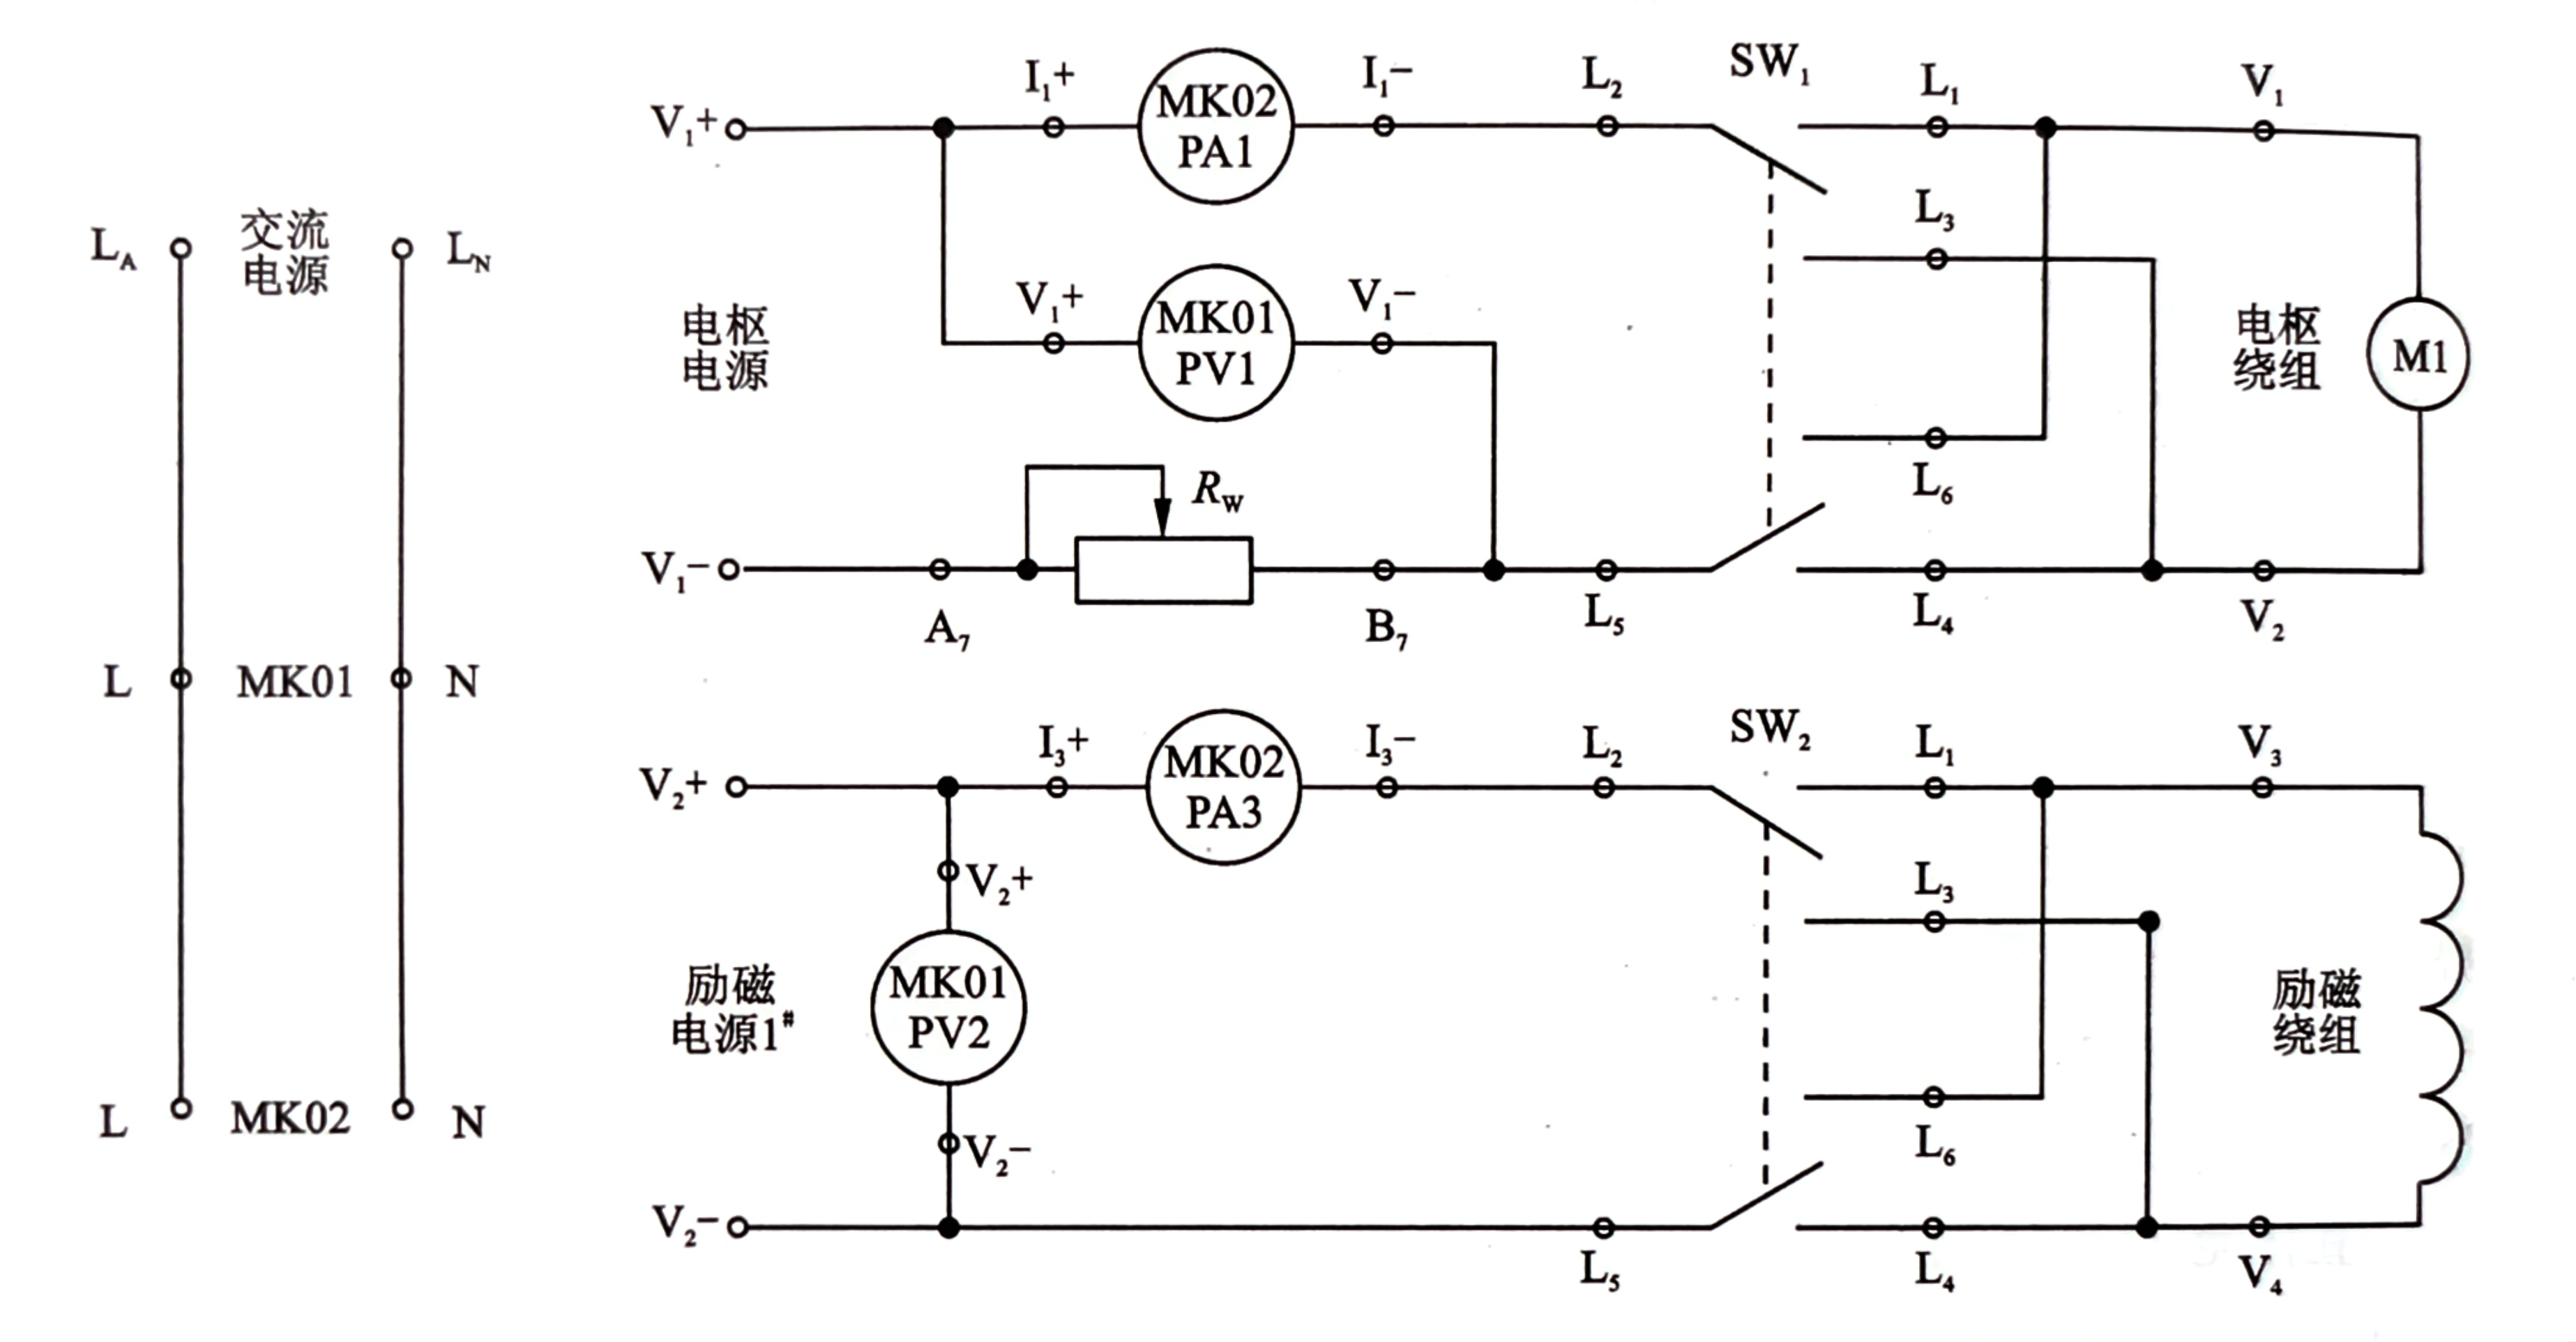
\includegraphics[width=0.8\textwidth]{fig2-3.jpg}
				\caption{\hspace{0.5em}直流他励电动机启动与换向实验接线图}
			\end{figure}
			
			\subsection{直流他励发电机的空载特性实验、直流他励发电机的负载特性实验}
			空载特性描述的是发电机在无负载（$I_L=0$）且维持额定转速（$n=n_N$）的前提下，输出端电压随励磁电流变化的规律 $U_0 = f(I_f)$。负载特性即外特性，则表征在转速与励磁电流均保持恒定时，发电机输出电压与负载电流之间的函数关系 $U = f(I_L)$。
			
			\begin{figure}[H] 
				\centering
				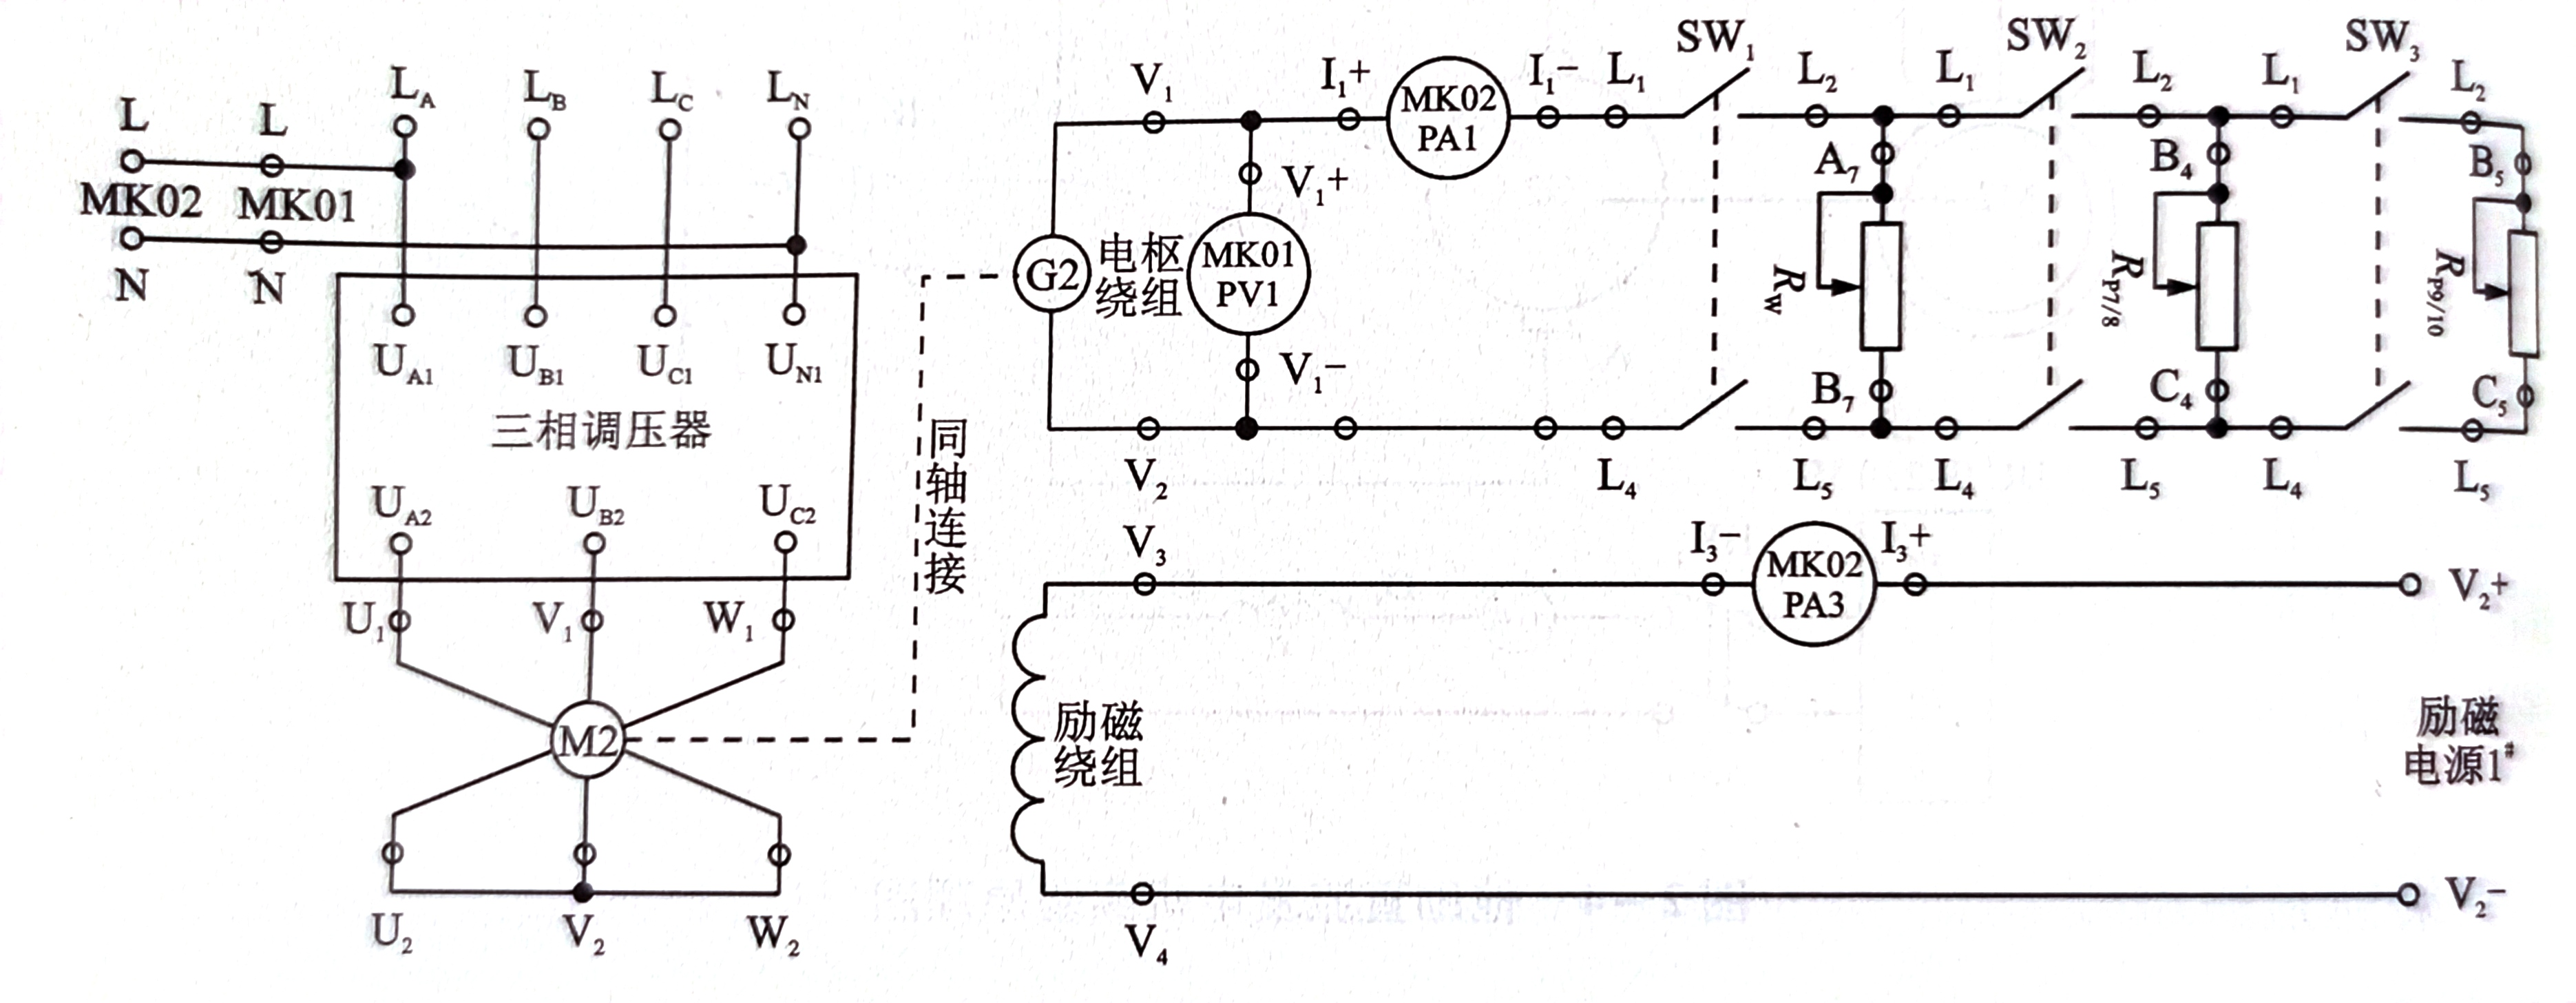
\includegraphics[width=0.8\textwidth]{fig2-6.jpg}
				\caption{\hspace{0.5em}直流他励发电机实验接线图}
			\end{figure}
			
			\subsection{他励直流电动机运行特性实验}
			运行特性侧重考察电机在额定电压 $U=U_N$ 与额定励磁 $I_f = I_{fN}$ 工况下，其转速 $n$ 随电枢电流即负载大小 $I_a$ 变动的轨迹，即 $n = f(I_a)$。
			
			\begin{figure}[H] 
				\centering
				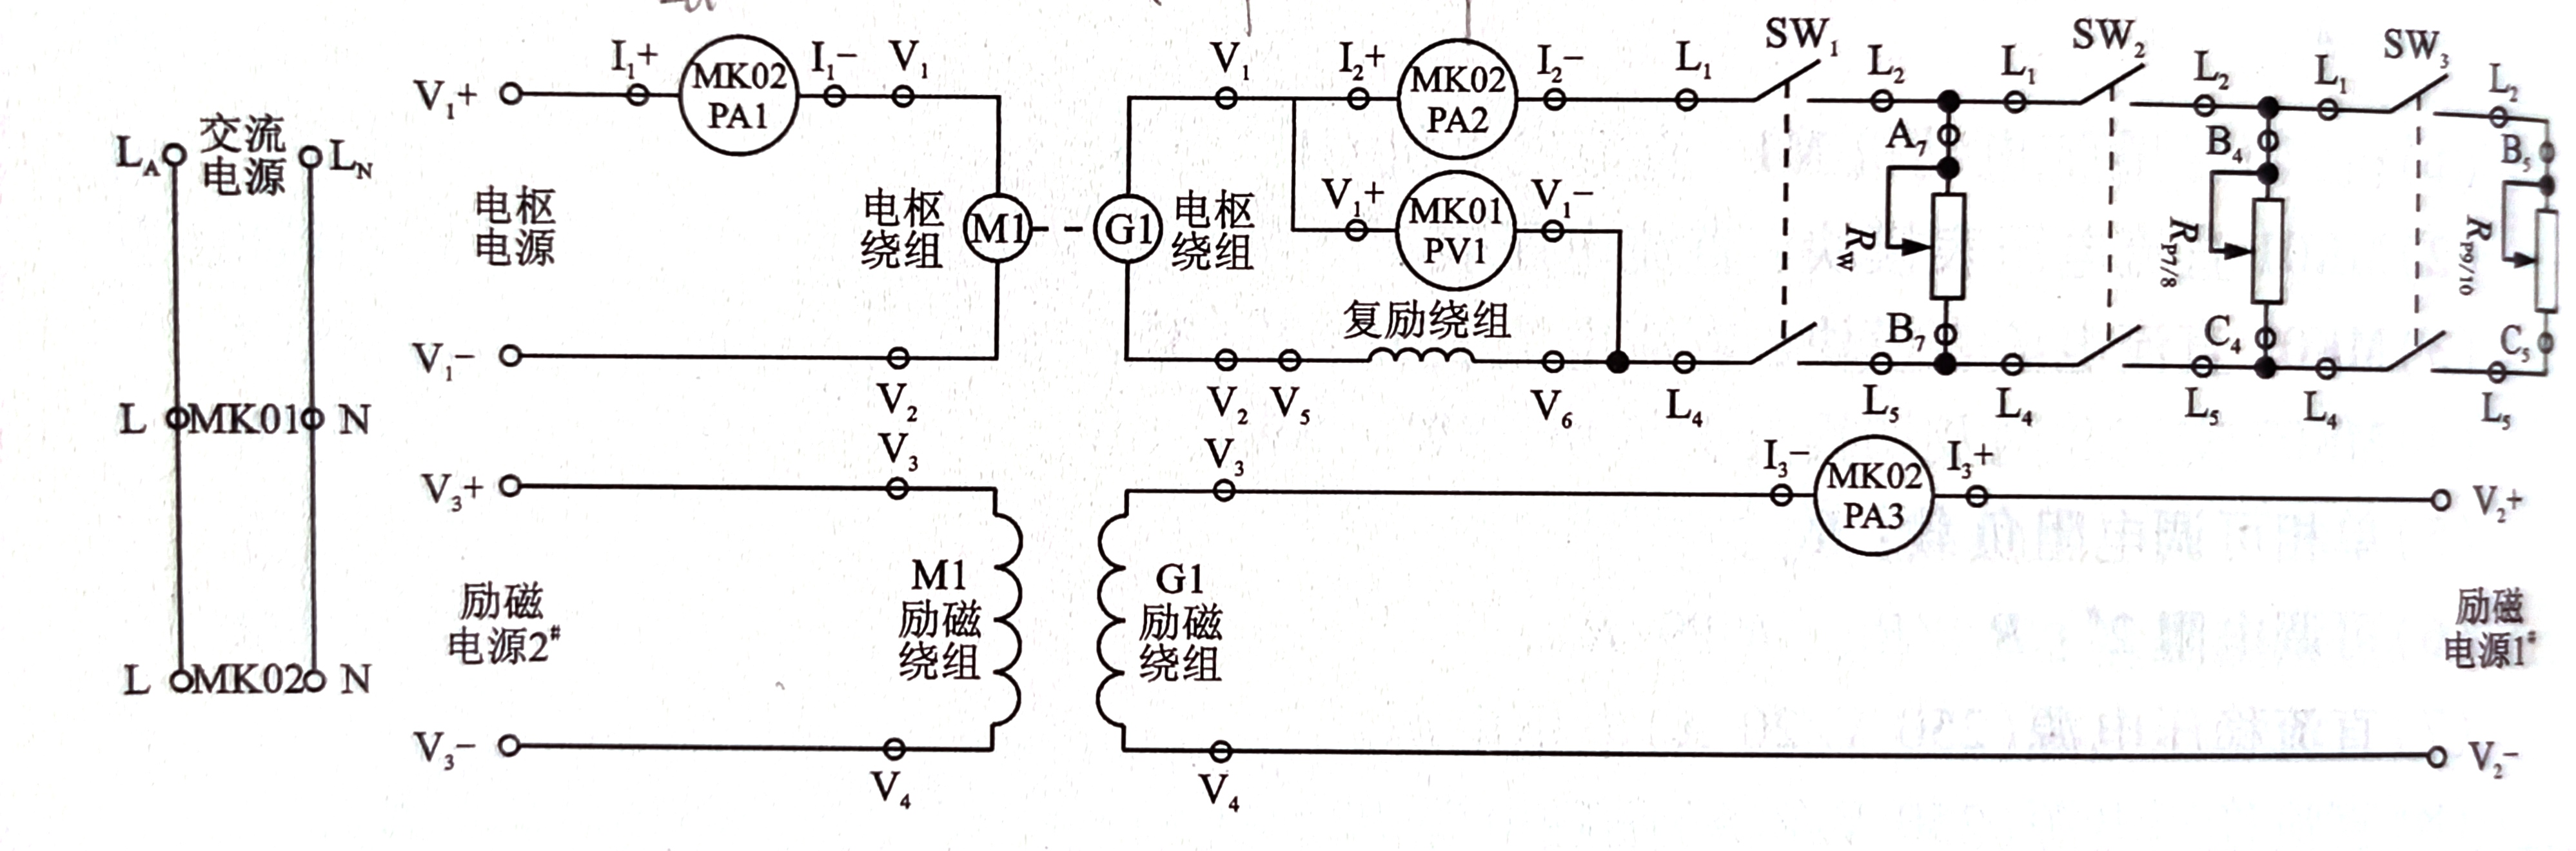
\includegraphics[width=\textwidth]{fig2-10.jpg}
				\caption{\hspace{0.5em}他励直流电动机实验接线图}
			\end{figure}
			
			\section{实验步骤和说明}
			
			\subsection{直流电动机的启动、换向和调速控制实验}
			
			\subsubsection{直流电动机的启动与换向}
			\begin{enumerate}
				\item 依照原理图完成接线，确保启动电阻及调压旋钮处于安全初始位。
				\item \textbf{开机操作规范：}务必优先接通励磁电源以建立最大主磁通，随后方可闭合电枢电源进行启动，以此防范电机超速失控危险。
				\item 待系统平稳后断电。分别测试并记录单独反转电枢极性与单独反转励磁极性时的电机旋转方向变化。
			\end{enumerate}
			
			实验数据：
			\begin{table}[H]
				\centering
				\caption{\hspace{0.5em}直流电动机换向记录表}
				\begin{tabular}{ccccc}
					\toprule
					$\text{SW}_1$ & $\text{SW}_2$ & 电枢电源极性 & 励磁电源极性 & 电机转向 \\
					\midrule
					左侧 & 左侧 & 正 & 正 & 正向 \\
					左侧 & 右侧 & 正 & 负 & 负向 \\
					右侧 & 右侧 & 负 & 正 & 正向 \\
					右侧 & 左侧 & 负 & 负 & 负向 \\
					\bottomrule
				\end{tabular}
			\end{table}
			
			\subsubsection{直流电动机的调速}
			调节电枢电压能够达成平滑的无级调速效果，该方式不会改变机械特性的硬度，且调速区间宽广，非常契合恒转矩负载的需求。
			\begin{enumerate}
				\item 依图连线，利用专用线缆将转速表接口与1号机组测速端相连。
				\item 把 $R_W$ 逆时针旋至阻值下限，同时将 $\text{SW}_1$ 与 $\text{SW}_2$ 拨至左侧位置。
				\item 借助上位机软件接通系统，依次开启交流总闸、直流总闸、电枢电源开关及1号励磁电源开关。
				\item 设定1号励磁电源输出，使励磁电流稳定在额定参数0.43A，随后逐步调节电枢电压，并将对应读数填入表格。
			\end{enumerate}
			
			\begin{table}[H]
				\centering
				\caption{\hspace{0.5em}电枢电压与转速关系}
				\begin{tabular}{cccccccc}
					\toprule
					电枢电压(V) & 70 & 90 & 110 & 130 & 150 & 170 & 190 \\
					\midrule
					转速($\mathrm{r} \cdot \mathrm{min}^{-1}$) & 561 & 727 & 889 & 1058 & 1225 & 1386 &1551 \\
					\bottomrule
				\end{tabular}
			\end{table}
			
			\subsection{直流他励发电机的空载特性实验}
			操作指引：利用电动机带动发电机达到额定转速 $n=n_N$。在输出端开路（$I_L=0$）状态下，单向递增发电机的励磁电流 $I_f$，从零逐渐升至峰值，同步记录发电机空载电压 $U_0$ 与 $I_f$ 的对应数值。实验数据：
			\begin{table}[H]
				\centering
				\caption{\hspace{0.5em}发电机空载特性实验数据 ($n=n_N, I_L=0$)}
				\begin{tabular}{cccccccccc}
					\toprule
					序号 & 1 & 2 & 3 & 4 & 5 & 6 & 7 & 8 & 9\\
					\midrule
					$I_f$ (A) & 0 & 0.026 & 0.079 & 0.111 & 0.156 & 0.178 & 0.201 & 0.245 & 0.264\\
					$U_0$ (V) & 34.9 & 54.4 & 119.4 & 147.1 & 190.9 & 206.8 & 221.6 & 244.1 & 252.6\\
					\bottomrule
				\end{tabular}
			\end{table}
			
			\subsection{直流他励发电机的负载特性实验}
			\textbf{操作指引：}维持发电机转速 $n=n_N$ 及励磁电流恒定。闭合负载侧开关，通过旋动可调电阻 $R_W$ 来逐步降低负载阻值，观测并记录端电压 $U$随负载电流 $I_L$ 增加而发生的变化。
			
			\textbf{实验数据：}
			\begin{table}[H]
				\centering
				\caption{\hspace{0.5em}发电机负载(外)特性实验数据$n=n_N=1456\text{r/min}$，$I=I_fN=0.253\text{A}$}
				\begin{tabular}{cccccccc}
					\toprule
					& 1 & 2 & 3 & 4 & 5 & 6 & 7 \\
					\midrule
					记录点 & $I_L=3.5\text{A}$ & & & $R_W=\text{最大值}$ & 断开$\text{SW}_3$ & 断开$\text{SW}_2$ & 断开$\text{SW}_1$ \\
					$U$ (V) & 177.6 & 182.9 & 185.9 & 192.5 & 205.6 & 216.9 & 221.9 \\
					$I_L$ (A) & 3.562 & 3.266 & 3.078 & 2.723 & 1.805 & 0.722 & 0.183 \\
					\bottomrule
				\end{tabular}
			\end{table}
			
			\subsection{他励直流电动机运行特性实验}
			\textbf{操作指引：}调整发电机侧负载，促使电动机进入满载工况，并确保电动机端电压 $U=U_N$ 且 $I_f$ 处于额定水平。随后依次断开 $\text{SW}_3$、$\text{SW}_2$、$\text{SW}_1$ 以阶梯式减轻电动机轴上的机械负荷，同步记录电枢电流 $I_a$ 与转速 $n$ 的数据。
			
			\textbf{实验数据：}
			\begin{table}[H]
				\centering
				\caption{\hspace{0.5em}他励直流电动机运行特性实验数据$n=n_N=1490\mathrm{r} \cdot \mathrm{min}^{-1}$，$R_{f2}=\text{常数}$}
				\begin{tabular}{cccccccc}
					\toprule
					& 1 & 2 & 3 & 4 & 5 & 6 & 7 \\
					\midrule
					记录点 & $I_d=6.8\text{A}$ & & & $R_W=\text{最大值}$ & 断开$\text{SW}_3$ & 断开$\text{SW}_2$ & 断开$\text{SW}_1$ \\
					$I_d$ (A) & 6.564 & 6.338 & 6.118 & 5.968 & 3.947 & 1.872 & 0.754 \\
					$I_f$ (A) & 3.520 & 3.393 & 3.260 & 3.182 & 2.045 & 0.781 & 0.001 \\
					$N$($\mathrm{r} \cdot \mathrm{min}^{-1}$) & 1332 & 1337 & 1344 & 1347 & 1397 & 1445 & 1474 \\
					\bottomrule
				\end{tabular}
			\end{table}
			
			\section{实验结果和结论}
			\subsection{数据结果分析}
			综合上述采集的实验数据，可提炼出如下物理规律：
			\begin{itemize}
				\item \textbf{发电机空载特性：}伴随励磁电流 $I_f$ 的提升，空载电压 $U_0$ 呈现递增态势。该曲线在起始阶段具备良好的线性特征，随后受铁芯磁路饱和效应影响而趋于平缓。当 $I_f=0$ 时，因定子铁芯残留磁性的存在，依然可测得34.9V的空载电压。
				\item \textbf{发电机外特性：}随着负载电流 $I_L$ 的攀升，发电机输出端电压 $U$ 出现显著的下滑。导致该现象的核心因素在于电枢回路内阻产生的电压损耗（$I_L R_a$）以及电枢反应所引发的去磁效应。
				\item \textbf{电动机运行特性：}在负载逐步卸载的过程中，即电枢电流 $I_a$ 由6.752A回落至0.754A时，电动机转速 $n$ 仅从1332 r/min轻微攀升至1508 r/min。整个测试区间内转速波动幅度极小，这充分印证了他励直流电机具备高硬度机械特性的理论推断。
			\end{itemize}
			
			\subsection{问题探讨}
			\textbf{1. 为什么发电机的电磁转矩就是电动机的负载转矩？}
			
			答：在本次测试所采用的M-G机组中，直流电动机与发电机依托联轴器实现了同轴刚性连接。当发电机接入电气负载后，其电磁机制会产生一种阻碍转子运动的制动转矩。因此，对于提供动力的电动机而言，克服发电机内部的这种电磁制动作用，在物理意义上完全等效于克服其输出轴上的机械负载。
			
			\vspace{1em}
			
			\textbf{2. 怎样才能改变直流电动机的旋转方向？}
			
			答：依据直流电机的电磁转矩表达式 $T = C_T \Phi I_a$ 可以推断，若要实现电机反转即转矩反向，必须且仅能调整以下两个变量之一：其一是翻转主磁通 $\Phi$ 的方向，这通过对调励磁电源极性来实现；其二是改变电枢电流 $I_a$ 的流向，这需要对调电枢供电极性。假若两者被同时反转，电磁转矩的最终方向将维持原状，电机转向亦不会改变。
			
			\vspace{1em}
			
			\textbf{3. 为什么减小 $R_z$，会使电动机的电枢电流加大？}
			
			答：在当前的电动机与发电机联调系统中，电阻 $R_z$ 即指导书中的 $R_W$ 代表连接于发电机输出端的负载电阻。调低 $R_z$ 促使电动机电枢电流攀升的内在机理如下：
			\begin{enumerate}
				\item \textbf{发电机电气负荷加重：}当负载电阻 $R_z$ 减小时，遵循欧姆定律，发电机的输出电流即负载电流 $I_L = U_G / R_z$ 必然增大。
				\item \textbf{发电机电磁阻力剧增：}发电机电枢电流上升后，其内部诱发的电磁转矩 $T_G = C_T \Phi_G I_L$ 同步增强。对发电机自身而言，这表现为更强的制动阻力。
				\item \textbf{电动机机械负担加剧：}鉴于两台电机同轴相连，发电机的制动转矩会直接转化为电动机轴端的机械负载转矩 $T_L$。
				\item \textbf{转速微降与反电动势衰减：}电动机面临更大的负载转矩，打破了原有的力学平衡，迫使转速 $n$ 产生微幅下降。依据公式 $E_a = C_e \Phi n$，转速的降低会直接导致电动机反电动势 $E_a$ 减弱。
				\item \textbf{电枢电流自发补偿：}根据电动机电压平衡方程 $I_a = \frac{U - E_a}{R_a}$，在外部供电电压 $U$ 与电枢内阻 $R_a$ 恒定的前提下，反电动势 $E_a$ 的衰减势必促使电枢电流 $I_a$ 自动攀升，直至电机输出的电磁转矩足以抗衡新的负载转矩，系统方能重新建立平衡。
			\end{enumerate}
			
			\vspace{1em}
			
			\textbf{4. 直流电动机的运行特性包括哪些？如何用实验方法求取这些特性？}
			
			答：他励直流电机的运行特性，是指在确保电机端电压等于额定值 $U_N$ 的前提下，电机的各项核心参数随负载演变的规律，负载通常用电枢电流 $I_a$ 或输出功率 $P_2$ 衡量。具体涵盖：
			\begin{itemize}
				\item \textbf{转速特性：}$n = f(I_a)$，揭示转速随负载电流波动的趋势。
				\item \textbf{转矩特性：}$T = f(I_a)$，展现电磁转矩随电枢电流变化的关联。
				\item \textbf{效率特性：}$\eta = f(P_2)$，反映电机能量转换效率随输出功率变化的轨迹。
			\end{itemize}
			\textbf{实验测定途径：}
			\begin{enumerate}
				\item \textbf{确立基准状态：}调节电枢供电使端电压稳定在 $U_N$，同时设定励磁电流至 $I_{fN}$，并确保这两项参数在整个测试周期内绝对恒定。
				\item \textbf{动态调整负载：}借助调节同轴发电机的负载电阻，使电动机的运行工况从空载平滑过渡至1.2倍额定负载左右。
				\item \textbf{采集关键数据：}在每一个负载稳定点，准确读取并记录电动机的电枢电流 $I_a$、端电压 $U$、输入功率 $P_1$、实时转速 $n$ 以及轴端输出转矩 $T_2$。
				\item \textbf{绘制特性图谱：}将获取的离散坐标点导入直角坐标系并进行平滑连接，即可得到直观的运行特性曲线。
			\end{enumerate}
			
			\vspace{1em}
			
			\textbf{5. 何谓直接启动？为什么直流电动机不能直接启动？}
			
			答：\textbf{直接启动}是指在电机转子静止即 $n=0$ 的状态下，不采取任何限流辅助手段，径直将电枢绕组接入额定电压 $U_N$ 电网的启动操作。
			
			除极少数微型电机外，常规直流电机严禁采用直接启动方式，具体缘由如下：
			\begin{enumerate}
				\item \textbf{启动电流极度超标：}依据电枢电流方程 $I_a = \frac{U - E_a}{R_a}$，通电瞬间转子尚未旋转，反电动势 $E_a = 0$。此时启动电流高达 $I_{st} = \frac{U_N}{R_a}$。由于电机设计时为降低运行铜耗，电枢内阻 $R_a$ 极小，这会导致直接启动电流飙升至额定值的10至20倍甚至更高。
				\item \textbf{损毁换向装置：}如此庞大的电流冲击会在换向器与电刷接触面激发出剧烈的电火花，极易诱发环形电弧故障，从而在瞬间烧毁换向器。
				\item \textbf{诱发破坏性机械应力：}超大电流会伴生极其猛烈的冲击性电磁转矩，对电机主轴、轴承及后级传动机构造成不可逆的机械破坏，例如扭断电机转轴。
				\item \textbf{严重干扰供电网络：}巨额的启动电流会拉低电网电压，造成线路电压瞬时大幅跌落，进而危及同一供电网络内其他用电设备的运行安全。
			\end{enumerate}
			
			基于上述危害，直流电机启动时必须引入降压机制或在电枢回路串接限流电阻。
			
		}
	\end{framed}
\end{document}